\section{Bargaining over color-group completion}
\label{sec:bargaining}

\subsection{The negotiation population}

The twenty games contain 526 negotiation threads and 920 response opportunities. Recipients accept 113 offers, counter 394 and reject 413. In two cases the engine does not offer acceptance, because accepting would leave a party with negative cash after transfer interest; excluding them leaves 918 acceptance-legal offers for comparisons that require a real choice to accept. Threads are short. The median thread has one response, the longest has eleven counters, and none spans a new global turn. Players return to the same partners often: 414 of 526 threads follow an earlier thread between the same pair in the same game.

The 113 settlements complete a color group for neither party in 60 cases, for one party in 43 and for both in 10, giving the 63 trade-completed groups followed in Section~\ref{sec:construction}. In 44 settlements the final terms were written by the player who did not start the thread, so assigning settled bundles to the initiator would misdescribe who proposed what.

\subsection{Rival completion is refused or priced}
\label{sec:rival}

\begin{figure}[htbp]
\centering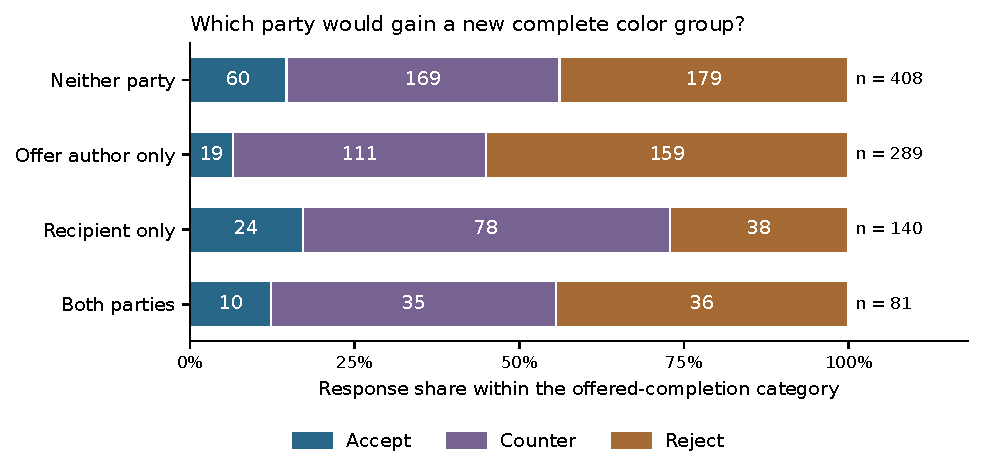
\includegraphics[width=0.92\linewidth]{offer_responses.pdf}
\caption{Responses to all 918 acceptance-legal offers, grouped by which party would gain a newly complete color group if the offer were accepted. ``Offer author'' is the writer of the current terms, not the thread initiator. Offers within a thread, pair and game are dependent observations.}
\label{fig:offers}
\end{figure}

Offers that would complete only the author's group fare worst (Figure~\ref{fig:offers}). Recipients accept 19 of 289 (6.6\%) and reject 159 (55\%), although the median such offer pays the recipient \$200 net. Offers that would complete only the recipient's group are accepted 24 times in 140 (17\%) and rejected 38 times (27\%), although the median one asks the recipient to pay \$350. Offers completing neither party fall between (60 accepted and 179 rejected of 408), and offers completing both are accepted 10 times in 81. Within the author-only cell, cash barely separates outcomes: the median payment to the recipient is \$200 for accepted offers, \$230 for countered offers and \$180 for rejected ones.

What recipients do when they counter says more than how often they reject. Table~\ref{tab:counters} compares each counter with the offer it answers. Of 111 counters to author-only offers, 92 keep the author's completion. In 88 of these the counterer gains no group of its own, and 85 of the 88 ask for more cash, with a median increase of \$125. Thirteen counters replace the deal with one that completes the counterer's group instead and pay for it. Only six strike the completion and give neither side a group.

\begin{table}[htbp]
\centering\small
\setlength{\tabcolsep}{4pt}
\begin{tabular}{@{}llrrr@{}}
\toprule
Offer answered & What the counteroffer does & Counters & Cash rises & Median change\\
\midrule
\multirow{4}{*}{Author only (111)} & Keeps author's completion only & 88 & 85 & $+$\$125\\
 & Keeps author's and adds counterer's & 4 & 2 & $+$\$100\\
 & Swaps to counterer's completion & 13 & 0 & $-$\$560\\
 & Removes all completion & 6 & 2 & \$0\\
\midrule
Recipient only (79) & Keeps counterer's completion & 78 & 77 & $+$\$122.5\\
Both (35) & Keeps both completions & 29 & 26 & $+$\$143\\
Neither (169) & Neither completes & 164 & 135 & $+$\$75\\
\bottomrule
\end{tabular}
\caption{What counteroffers change, for all 394 counters. ``Counterer'' is the recipient of the offer being answered; cash change is its net cash under the counteroffer minus its net cash under the offer answered. Rows omit cells with fewer than two counters (one recipient-only counter, six ``both'' counters that drop the author's completion and five ``neither'' counters that add the counterer's). The recipient-only row includes one counter to an offer for which acceptance was not legal. Source: \texttt{data/opus\_retabulation.json}.}
\label{tab:counters}
\end{table}

Counters in every cell usually ask for more cash, including 135 of 164 counters that involve no completion, so the premium itself is ordinary bargaining. What is specific is that the completing deed stays on the table: recipients who keep negotiating over a rival's completion almost always negotiate its price rather than its existence. Thread outcomes point the same way. Of 187 threads whose opening offer would complete only the initiator's group, 26 settle, and in 24 of these the initiator still completes its group after raising its cash offer by a median \$97.50. Threads that open with an offer completing the recipient's group settle 17 times in 53.

In this population a rival's completion is something recipients refuse or charge for. This is the observational counterpart of the first research question's example: agents do turn down trades that hand an opponent a dangerous advantage, including trades that pay them. The ledger cannot show that any refusal was correct, that the premiums were efficient, or that rival completion caused the responses. The offers differ in price, deeds, timing and position, and repeated threads make the observations dependent.

\subsection{Configurations resist in different ways}
\label{sec:config-heterogeneity}

\begin{table}[htbp]
\centering\small
\begin{tabular}{@{}lrrrrrr@{}}
\toprule
& \multicolumn{2}{c}{All responses} & \multicolumn{2}{c}{Accepted} & \multicolumn{2}{c}{Counters keeping author's}\\
& \multicolumn{2}{c}{} & \multicolumn{2}{c}{} & \multicolumn{2}{c}{completion only}\\
\cmidrule(lr){2-3}\cmidrule(lr){4-5}\cmidrule(lr){6-7}
Responder & Reject & Counter & Author only & Recipient only & Ask more & Median\\
\midrule
Sol & 65/235 & 140/235 & 2/83 & 6/30 & 35/36 & $+$\$150\\
Gemini & 180/242 & 36/242 & 4/76 & 6/31 & 7/7 & $+$\$130\\
Opus & 19/189 & 141/189 & 7/52 & 5/42 & 34/36 & $+$\$77.5\\
Grok & 149/254 & 77/254 & 6/78 & 7/37 & 9/9 & $+$\$260\\
\bottomrule
\end{tabular}
\caption{Response style by responding configuration. ``All responses'' uses all 920 opportunities; acceptance columns use acceptance-legal offers in the named cell. Opus responds under the action-only condition in 162 of its 189 opportunities. Appendix~\ref{app:offers} gives the full cell-by-configuration, seed-block and game tables.}
\label{tab:responders}
\end{table}

The pooled pattern hides two styles (Table~\ref{tab:responders}). Gemini and Grok mostly reject, Sol and Opus mostly counter, and Opus rejects only 19 times in 189. Reject counts therefore mix style with any sensitivity to completion, which is why we lead with acceptance and counter content.

Three configurations show the acceptance gradient: Sol accepts 2 of 83 author-only offers against 6 of 30 recipient-only offers, Gemini 4 of 76 against 6 of 31, and Grok 6 of 78 against 7 of 37. Opus does not, accepting 7 of 52 and 5 of 42. Its counters still price the rival's completion: 34 of the 36 that keep only the author's completion ask for more cash, with a smaller median increase (\$77.50) than the others. Because Opus answered 162 of its 189 offers under the action-only condition, its bargaining style cannot be separated from that condition.

The reject comparison points the same way in all five seed blocks and in 17 of the 19 games where both cells occur. The acceptance comparison is less stable and reverses in block~3 (5 of 57 author-only offers accepted against 1 of 24 recipient-only offers). These are consistency checks on dependent, unequal cells, not tests of a causal effect; game~1 alone contributes 25 author-only offers.

\subsection{Stated reasons and roles}

All 74 direct rejections of offers that would complete the recipient's own group have public text, and 66 have a private note. Two LLM readers agree that 61 state a trade-linked consequence for the rival, such as completing its group or funding its houses (Section~\ref{sec:coding}). Their four disagreements turn on whether a cash transfer alone implies funding a rival and whether an inferred consequence counts as stated, and two notes adopt the wrong buyer or seller role (G15 d106, G17 d186). The readings describe stated considerations; they do not verify the arithmetic or show that the consideration caused the rejection.

Initiation also differs. Opus proposes on 160 of its 660 eligible own turns, Grok on 106 of 676, Sol on 83 of 834 and Gemini on 16 of 766. Gemini's 18 proposals settle 11 times and Opus's 240 settle 44 times. Selective proposing, inventory and opponents' demands could each produce these differences, and none of the counts measures bargaining quality (Appendix~\ref{app:offers}).

\subsection{Two bargaining incidents}

\Incident{g2}{A completion priced, refused, and later sold in reverse (G2)}
\Setup{At turn 45 of game 2, Opus (p4) holds Atlantic and Ventnor and has \$845. Sol (p1) holds Marvin Gardens, the third yellow, and has \$161. Opus offers \$325 for Marvin, which would complete Opus's yellows. Both players respond under the standard prompt in this thread.}

\TranscriptQuote{g2-d124-price}
\TranscriptQuote{g2-d124-note}

Opus counters at \$400 and Sol at \$600. Opus then writes:

\TranscriptQuote{g2-d127-final}
\TranscriptQuote{g2-d127-ceiling}

Sol answers:

\TranscriptQuote{g2-d128-keep}

At turn 69 the direction reverses. Sol offers two railroads for Atlantic and Ventnor, which would complete Sol's yellows. Opus, now under the action-only condition, counters, and Sol accepts:

\TranscriptQuote{g2-d197-reverse}
\TranscriptQuote{g2-d198-note}

\TranscriptFinding{The turn-45 thread ends without a trade. At turn 69 Sol receives Atlantic and Ventnor for the railroads and \$100. Sol spends \$300 on yellow houses, collects no rent on them and recovers \$150 in sales. At d239 it holds \$77 against \$1,300 of Park Place rent owed to Gemini and is eliminated. Gemini inherits the yellow group, spends \$900 more on it and wins the game.}

\TranscriptReading{Both sides reason about the other's building cash after the trade. Sol computes what Opus would keep at \$325 and at \$650, and Opus argues from Sol's thin cash; since cash is public, these are capacity calculations rather than inferences about hidden beliefs. Opus's ``final'' \$450 sits below its private \$475 ceiling, an authorized bluff that ends the thread, so whether Sol would have sold at \$475 is unknown. The sequence shows the whole chain studied here: a completion is first priced, then sold in the other direction, built on without return, and passed through bankruptcy to the eventual winner. It does not show that any party misjudged the trade.}

\TranscriptSource{G2 d124--128 (turn 45) and d197--198 (turn 69). Every quoted message appears in the recipient's next prompt. Spans, hashes and line numbers are in \path{data/opus_quote_manifest.json}; outcomes come from the offer, flow, spending and elimination ledgers and the d239 events.}

\Incident{g11}{Refusing one's own completion because it completes the rival (G11)}
\Setup{Late in game 11 only Grok (p2) and Sol (p4) remain. Grok holds States Avenue and mortgaged Pennsylvania Avenue, which it inherited from Gemini's estate at turn 81. Sol holds North Carolina and Pacific, so Pennsylvania would complete Sol's greens, and it holds St.~Charles and Virginia. At d255 Sol offers Virginia for Pennsylvania plus \$150, claiming that Virginia completes Grok's pinks. The claim is false, because Grok lacks St.~Charles.}

\TranscriptQuote{g11-d256-public}

Sol concedes the error and offers both St.~Charles and Virginia for Pennsylvania plus \$250, which would genuinely complete Grok's pinks.

\TranscriptQuote{g11-d258-public}
\TranscriptQuote{g11-d258-note}

\TranscriptFinding{Pennsylvania never changes hands while Sol is alive, and Sol never completes the greens. Sol pays Grok \$2,000 on Boardwalk at turn 125, is eliminated at d325 owing \$1,100, and its greens and pinks pass to Grok in the final estate. Grok wins the game.}

\TranscriptReading{This is the first research question's example in its plainest form: an agent declines a trade that completes its own group because the same trade completes the rival's. The note's liquidation estimate for Sol is not scored here, since the Boardwalk landing came 28 turns later at a different rent and Sol paid it. Grok's refusal at d256 also corrects a false premise, a correction its returned provider explanation reached only after first repeating the premise (Appendix~\ref{app:incidents}). The blocker itself came from an estate, which links the refusal to the inheritance results in Section~\ref{sec:inheritance}.}

\TranscriptSource{G11 d255--258 (turn 97), standard condition, selected attempt 0. Sol's false claim is in Grok's d256 prompt, and Grok's reply is in Sol's d257 prompt.}

\FloatBarrier
